\documentclass[12pt, a4paper, oneside]{ctexart}
\usepackage{amsmath, amsthm, amssymb, bm, color, graphicx, geometry, hyperref, mathrsfs,extarrows, braket, booktabs, array, listings, xcolor, fontspec, appendix}
\setmonofont{Consolas}

%%%%%% 设置字号 %%%%%%
\newcommand{\chuhao}{\fontsize{42pt}{\baselineskip}\selectfont}
\newcommand{\xiaochuhao}{\fontsize{36pt}{\baselineskip}\selectfont}
\newcommand{\yihao}{\fontsize{28pt}{\baselineskip}\selectfont}
\newcommand{\erhao}{\fontsize{21pt}{\baselineskip}\selectfont}
\newcommand{\xiaoerhao}{\fontsize{18pt}{\baselineskip}\selectfont}
\newcommand{\sanhao}{\fontsize{15.75pt}{\baselineskip}\selectfont}
\newcommand{\sihao}{\fontsize{14pt}{\baselineskip}\selectfont}
\newcommand{\xiaosihao}{\fontsize{12pt}{\baselineskip}\selectfont}
\newcommand{\wuhao}{\fontsize{10.5pt}{\baselineskip}\selectfont}
\newcommand{\xiaowuhao}{\fontsize{9pt}{\baselineskip}\selectfont}
\newcommand{\liuhao}{\fontsize{7.875pt}{\baselineskip}\selectfont}
\newcommand{\qihao}{\fontsize{5.25pt}{\baselineskip}\selectfont}

%%%% 下面的命令重定义页面边距,使其符合中文刊物习惯 %%%%
%\addtolength{\topmargin}{-54pt}
%\setlength{\oddsidemargin}{0.63cm}  % 3.17cm - 1 inch
%\setlength{\evensidemargin}{\oddsidemargin}
%\setlength{\textwidth}{14.66cm}
%\setlength{\textheight}{25.50cm}    % 24.62
%\geometry{left=1.84cm,right=1.84cm,top=2.18cm,bottom=2.18cm}
\geometry{left=2.54cm,right=2.54cm,top=3.18cm,bottom=3.18cm}

%%%% 代码块的基本设置 %%%%
\lstset{
    language = MATLAB,
    breaklines,%自动换行
    columns=flexible,%不随便添加空格,只在已经有空格的地方添加空格,
    %如果想要添加空格使用fixed作为参数(这是默认的),如果坚决不添加空格使用fullflexible作为参数.
    numbers=left, 
    numberstyle=\tiny,
    keywordstyle=\color{blue!70},
    commentstyle=\color{red!50!green!50!blue!50},
    frame=shadowbox,
    rulesepcolor=\color{red!20!green!20!blue!20},
    basicstyle=\ttfamily
}

%%%% 正文开始 %%%%
\begin{document}

%%%% 定理类环境的定义 %%%%
\newtheorem{example}{例}             % 整体编号
\newtheorem{algorithm}{算法}
\newtheorem{theorem}{定理}[section]  % 按 section 编号
\newtheorem{definition}{定义}
\newtheorem{axiom}{公理}
\newtheorem{property}{性质}
\newtheorem{proposition}{命题}
\newtheorem{lemma}{引理}
\newtheorem{corollary}{推论}
\newtheorem{remark}{注解}
\newtheorem{condition}{条件}
\newtheorem{conclusion}{结论}
\newtheorem{assumption}{假设}

%%%% 重定义 %%%%
\renewcommand{\contentsname}{目录}  % 将Contents改为目录
\renewcommand{\abstractname}{摘要}  % 将Abstract改为摘要
\renewcommand{\refname}{参考文献}   % 将References改为参考文献
\renewcommand{\indexname}{索引}
\renewcommand{\figurename}{图}
\renewcommand{\tablename}{表}
\renewcommand{\appendixname}{附录}
\renewcommand{\algorithm}{算法}


%%%% 定义标题格式,包括title,author,affiliation,email等 %%%%
\title{数值分析上机试验报告\\观察高次插值多项式的龙格现象}
\author{吴天阳\\2204210460\\[2ex]
\xiaosihao 西安交通大学\\ \xiaosihao 数学与统计学院\\[2ex]
}
\date{2022年3月18日}

\maketitle % 设置上面是标题
\newpage
\tableofcontents % 创建目录,使用目录需要编译两次,并且不能删去编译产生的临时文件!!!

%%%% 以下部分是正文 %%%%  
\newpage
\section{问题描述}
给定函数
\begin{equation*}
 f(x) = \dfrac{1}{1+25x^2}\quad (-1\leqslant x\leqslant 1)   
\end{equation*}
取等距节点,构造牛顿插值多项式$N_5(x)$和$N_{10}(x)$及三次样条插值函数$S_{10}(x)$。分别将三种插值多项式与$f(x)$的曲线画在同一个坐标系上进行比较。(在\textbf{\ref{sec:buchong}\ 附录}中加入了$\text{Chebyshev}$插值法,与等距节点插值做对比)

\section{算法实现}
本次全部使用$\text{MATLAB}$进行编程,使用$\text{MATLAB}$编程的好处在于可以容易地绘制函数图像,可实现带参数的运算,可化简/展开多项式,除了这几个功能外的更高级的功能,如解方程组,求三次样条插值等功能均由本人实现,不依靠$\text{MATLAB}$自带的函数,下面先将本文将会用到的所有$\text{MATLAB}$的自带函数统一给出,并介绍其功能:
\begin{lstlisting}
    syms x % 定义参数x
    f = (x+1)^2+(x+1)^2; % 定义函数
    simplify(f); % 化简多项式
    expand(f); % 展开多项式
    vpa(f, 5); % 将多项式的分式系数转换为5位有效数字的小数系数
    subs(f, 5); % 求值f(5)
    plot(); % 绘图函数
    hold on % 实现在同一个画板上画多个图像
    legend(); % 设置曲线标签
    set(); % 设置图像字体大小
    size(); % 求出矩阵的大小
\end{lstlisting}
\textbf{注意}:由于$\text{MATLAB}$中所有矩阵的下标都是从$1$开始的,所以下文中介绍算法原理的时候,为了和程序相对应,下标都会从$1$开始。为统一结构,所有一维向量均为\textbf{列向量}。

所有算法的详细证明及结论请见课本\footnote{《数值分析》李乃成},本文主要介绍如何将课本中的计算过程进行适当的调整,转化为适用于编程的数学公式,进而给出可运行代码,并强调在编程中需要注意的一些细节问题。

实现的算法从易到难分别为求解三对角方程组的追赶法,$\text{Newton}$插值法,三次样条插值法,下文将分别对这三种算法实现做出详细的解释,每一部分都会有对应部分的代码块,完整的代码会在\textbf{\ref{sec:fulu}\ 附录}中给出。
\subsection{求解三对角方程组的追赶法}\label{subsec:chase}
此算法在三次样条插值法中将会用到,所以先实现此算法。
\subsubsection{问题描述}
求解三对角方程组$Ax=d$,即:
\begin{equation*}
    \left[\begin{matrix}
        a_{11}&a_{12}& & & \\
        a_{21}&a_{22}&a_{23}& & \\
        & \ddots &\ddots&\ddots& \\
        & & a_{n-1,n-2} & a_{n-1,n-1} & a_{n-1,n}\\
        & & & a_{n, n-1}& a_{nn}
    \end{matrix}\right]\left[\begin{matrix}
        x_1\\x_2\\ \vdots\\x_{n-1}\\x_n
    \end{matrix}\right]=\left[\begin{matrix}
        d_1\\d_2\\ \vdots\\ d_{n-1}\\ d_n
    \end{matrix}\right]
\end{equation*}
\subsubsection{LU分解求解}
对系数矩阵$A$进行$LU$分解即可,再令$Ux = y$,转化原方程组问题为
\begin{equation*}
    \begin{cases}
        Ly = d,\\Ux=y.
    \end{cases}
\end{equation*}

在计算$LU$分解的同时就可以将$y$一并求出,且由于三对角矩阵的性质,使得$LU$分解计算量大幅降低,所以该算法具有线性的复杂度。

\subsubsection{代码实现}
追赶法部分代码可以参考《数值分析》李乃成\ 第$36$面的伪代码。
\begin{lstlisting}
function x = chase(A, d) % A为系数矩阵,d为方程组右侧列向量
    [n, ~] = size(A);
    % 预分配内存,提高运算速度
    u = zeros(n, 1);
    l = zeros(n, 1);
    y = zeros(n, 1);
    % 参考课本第36面代码
    u(1) = A(1, 1);
    y(1) = d(1);
    for i = 2 : n
        l(i) = A(i, i-1) / u(i-1);
        u(i) = A(i, i) - l(i) * A(i-1, i);
        y(i) = d(i) - l(i) * y(i-1);
    end
    x(n) = y(n) / u(n);
    for i = n-1 : -1 : 1
        x(i) = (y(i) - A(i, i+1) * x(i+1)) / u(i);
    end
end
\end{lstlisting}
\subsection{Newton插值法}
\subsubsection{算法原理}
使用$\text{Newton插值法}$计算的核心在于求解差商表,在程序中用矩阵$\text{diff}$表示,为符合编程习惯,将课本上的差商表取转置存储,即
\begin{equation*}
    \text{diff} = \left[\begin{matrix}
        f[x_1]&f[x_2]&f[x_3]&\cdots&f[x_n]\\
        &f[x_1,x_2]&f[x_2,x_3]&\cdots&f[x_{n-1},x_n]\\
        & &f[x_1,x_2,x_3]&\cdots &f[x_{n-2},x_{n-1},x_n]\\
        & & & \ddots &\vdots\\
        & & & & f[x_1,x_2,\cdots,x_n]
    \end{matrix}\right]
\end{equation*}
利用差商的性质,从上至下递推求解差商表,递推式如下(记$\text{diff}_{ij} = a_{ij}$):
\begin{equation*}
    a_{ij}=
    \begin{cases}
        f(x_j),&\quad i = 1;\\
        \dfrac{a_{i-1,j}-a_{i-1,j-1}}{x_j-x_{j-i+1}}, &\quad i\geqslant 2.
    \end{cases}
\end{equation*}
再利用差商表点的对角线上的元素即可容易地求出$\text{Newton插值多项式}$,即
\begin{equation*}
    \begin{aligned}
        N_n(x) = &\ f[x_1]+f[x_1,x_2](x-x_1)+f[x_1,x_2,x_3](x-x_1)(x-x_2)+\cdots\\
                &\ +f[x_1,x_2,\cdots,x_n](x-x_1)(x-x_2)\cdots(x-x_{n-1})\\
                =&\sum_{i=1}^nf[x_1,x_2,\cdots x_i]\pi_{i-1}(x)
    \end{aligned}
\end{equation*}
\subsubsection{代码实现}
\begin{lstlisting}
% a为插值点列向量,b为插值点对应的函数值列向量
function N = Newton(a, b)
    [n, ~] = size(a);
    diff = zeros(n, n); % 初始化差商表
    diff(1, :) = b';
    syms x % 定义参数x
    now = 1; % 对应上文中的 pi(x)
    N = diff(1, 1);
    % 递推计算差商表,并同时计算出插值多项式N(x)
    for i = 2 : n
        for j = i : n
            diff(i, j) = (diff(i-1, j)-diff(i-1, j-1)) / (a(j) - a(j-i+1));
        end
        now = now * (x-a(i-1));
        N = N + diff(i, i) * now;
    end
    N = expand(N); % 展开插值多项式
    N = vpa(N, 5); % 将分式系数转化为小数系数
end
\end{lstlisting}

\subsection{三次样条插值}
三次样条插值法中有三种边界条件,分别为:二阶导数条件,一阶导数条件,周期条件。
下文中所使用的的边界条件为第一种,即边界点处的二阶导数作为已知条件。

三次样条插值的具体推导过程课本上已有详细介绍,这里不再阐述,这里主要介绍如何将课本上复杂的运算,转化为矩阵运算的方式,这样不仅能加快运算速度($\text{MATLAB}$对矩阵运算有优化),同时还能减少代码量。
\subsubsection{参数定义}
下面定义所用的参数名和课本基本保持一致。
\renewcommand\arraystretch{0.8} % 设置表格高度为原来的0.8倍
\begin{table}[!htbp] % table标准
    \centering % 表格居中
    \begin{tabular}{p{3cm}<{\centering}p{10cm}<{\centering}} % 设置表格宽度
    %\begin{tabular}{cc}
        \toprule
        参数名&定义\\
        \midrule
        $f(x)$ & 被插函数\\
        $[a,b]$ & 插值区间\\
        $\{x_1,x_2,\cdots, x_n\}$ & 插值点集合$x_i\in[a,b]\ (i=1,2,\cdots, n)$\\
        $y_i$ & 在$x_i$处的函数值$f(x_i)\ (i=1,2,\cdots, n)$\\
        $S(x)$ & $n$个插值节点对应的三次样条插值函数\\
        $S_i(x)$ & $S(x)$在区间$[x_{i-1},x_i]$上的限制$(i=2,3,\cdots,n)$\\
        $M_i$ & 在$x_i$处的插值函数的二阶导函数值$S''(x_i)$\\
        $h_i$ & 第$i$段插值区间长度$x_i-x_{i-1}\ (i=2,3,\cdots, n)$\\
        $\mu_i$ & 中间变量$h_i/(h_i+h_{i+1})\ (i=2,3,\cdots, n-1)$\\
        $\lambda_i$ & 中间变量$1-\mu_i\ (i=2,3,\cdots, n-1)$\\
        $d_i$ & 中间变量$6f[x_{i-1},x_i,x_{i+1}]\ (i=2,3,\cdots, n-1)$\\
        \bottomrule
    \end{tabular}
\end{table}

由$S(x)$的定义可知
\begin{equation*}
    S(x) = 
    \begin{cases}
        S_2(x),&\quad x\in[x_1,x_2];\\
        S_3(x),&\quad x\in(x_2,x_3];\\
        \quad \vdots&\quad\\
        S_n(x),&\quad x\in(x_{n-1},x_n].
    \end{cases}
\end{equation*}
为了简便运算,定义一些向量如下(其中$\boldsymbol{a},\boldsymbol{b},M_1,M_n$由函数传入参数直接给出):
\begin{equation*}
    \begin{aligned}
        \boldsymbol{a} =&\ \left[\begin{matrix}
            x_1&x_2&\cdots&x_n
        \end{matrix}\right]^T\\
        \boldsymbol{b} =&\ \left[\begin{matrix}
            y_1&y_2&\cdots&y_n
        \end{matrix}\right]^T\\
        \boldsymbol{S}(x) =&\ \left[\begin{matrix}
            S_2(x)&S_3(x)&\cdots&S_n(x)
        \end{matrix}\right]^T\\
        \boldsymbol{M} =&\ [\begin{matrix}
            M_1& M_2&\cdots& M_n
        \end{matrix}]^T\\
        \boldsymbol{h} =&\ [\begin{matrix}
            h_2&h_3&\cdots&h_n
        \end{matrix}]^T\\
        \boldsymbol{\mu} =&\ [\begin{matrix}
            \mu_2&\mu_3&\cdots&\mu_{n-1}
        \end{matrix}]^T\\
        \boldsymbol{\lambda} =&\ \left[\begin{matrix}
            \lambda_2&\lambda_3&\cdots&\lambda_{n-1}
        \end{matrix}\right]^T\\
        \boldsymbol{d} =&\ \left[\begin{matrix}
            d_2&d_3&\cdots&d_{n-1}
        \end{matrix}\right]^T\\
    \end{aligned}
\end{equation*}
根据课本上的推导,计算$\boldsymbol{S}(x)$应分为如下三步:计算定义的向量$\boldsymbol{h},\boldsymbol{\mu}, \boldsymbol{\lambda}, \boldsymbol{d}$(预处理);构造求解$\boldsymbol{M}$的方程组,利用追赶法求解该方程组;解出$\boldsymbol{S}(x)$。

下面根据该过程进行逐步解析:
\subsubsection{预处理}\label{subsubsec:yuchuli}
根据各向量的定义可得
\begin{equation*}
    \begin{aligned}
        \boldsymbol{h}=&\ \left[\begin{matrix}
            h_2&h_3&\cdots&h_n
        \end{matrix}\right]^T=\left[\begin{matrix}
            x_2-x_1&x_3-x_2&\cdots&x_n-x_{n-1}
        \end{matrix}\right]^T\\
        \mu_i =&\ \frac{h_i}{h_i+h_{i+1}}\ (i=2,3,\cdots, n)\\
        \boldsymbol{\lambda} =&\ 1-\boldsymbol{\mu}\\
        d_i =&\ 6f[x_{i-1},x_i,x_{i+1}]=\frac{6}{h_{i+1}+h_i}\left(\frac{y_{i+1}-y_i}{h_{i+1}}-\frac{y_i-y_{i-1}}{h_i}\right)
    \end{aligned}
\end{equation*}

由于$d_i$的计算比较复杂,所以将由$h_i,h_{i+1}$构成的向量分别定义为$\boldsymbol{h_1},\boldsymbol{h_2}$,详细的代码如下
\begin{lstlisting}
    % a为传入的插值点构成的向量,b为插值点对应函数值构成的向量
    h = a(2:n) - a(1:n-1); % 求解向量h
    mu = h(1:n-2) ./ (h(1:n-2) + h(2:n-1)); % 求解向量mu
    la = 1 - mu; % 求解向量lambda
    h1 = h(1:n-2); % 定义中间变量h1
    h2 = h(2:n-1); % 定义中间变量h2
    % 求解向量d
    d = 6*((b(3:n)-b(2:n-1))./h2-(b(2:n-1)-b(1:n-2))./h1)./(h1+h2);
\end{lstlisting}

\subsubsection{构造并求解方程组}
这里直接使用第一种边界条件所构造的方程组$A\boldsymbol{x}=\boldsymbol{d}$如下\footnote{见《数值分析》李乃成\ 第135面(4,6,9')式}:
\begin{equation*}
    \left[\begin{matrix}
        2&\lambda_2& & & \\
        \mu_3&2&\lambda_3& & \\
        &\ddots&\ddots&\ddots& &\\
        & &\ddots&\ddots&\ddots& \\
        & & &\mu_{n-2}&2&\lambda_{n-2}\\
        & & & &\mu_{n-1}&2
    \end{matrix}\right]
    \left[\begin{matrix}
        M_2\\M_3\\\vdots\\M_{n-2}\\M_{n-1}
    \end{matrix}
    \right]=\left[\begin{matrix}
        d_2-\mu_2M_1\\d_3\\\vdots\\d_{n-2}\\d_{n-1}-\lambda_{n-1}M_n
    \end{matrix}\right]
\end{equation*}
利用循环的方式即可生成系数矩阵$A$,右侧列向量$\boldsymbol{d}$可以直接修改在\textbf{\ref{subsubsec:yuchuli}}\textbf{预处理}步骤中所得到的$\boldsymbol{d}$,使用上文的$\textbf{\ref{subsec:chase}求解三对角方程组的追赶法}$即可解出$M_2,M_3,\cdots,M_{n-1}$,最后将边界条件$M_1,M_{n}$带入,即可求出$\boldsymbol{M}$。

具体代码实现如下:
\begin{lstlisting}
    A = zeros(n-2, n-2); % 初始化系数矩阵A
    for i = 1 : n-2 % 循环构造系数矩阵A
        if (i > 1)
            A(i, i-1) = mu(i); % 对角线下方
        end
        A(i, i) = 2; % 对角线
        if (i < n-2)
            A(i, i+1) = la(i); % 对角线上方
        end
    end
    % M1,Mn为对应传入的两个边界条件
    d(1) = d(1) - mu(1) * M1; % 修改向量d
    d(n-2) = d(n-2) - la(n-2) * Mn; % 修改向量d
    M = [M1; chase(A, d)'; Mn]; % 利用追赶法求解方程组,并解出向量M
\end{lstlisting}
\subsubsection{求出插值函数S(x)}
这里直接给出插值函数表达式,如下\footnote{见《数值分析》李乃成\ 第133面(4.6.3)式}:
\begin{equation*}
    \begin{aligned}
        S_i(x) =&\ \frac{(x_i-x)^3}{6h_i}M_{i-1}+\frac{(x-x_{i-1})^3}{6h_i}M_i\\
        &+\left(y_{i-1}-\frac{h_i^2}{6}M_{i-1}\right)\frac{x_i-x}{h_i}+\left(y_i-\frac{h_i^2}{6}M_i\right)\frac{x_i-x_{i-1}}{h_i}
    \end{aligned}\quad (i=2,3,\cdots, n)
\end{equation*}
如果直接计算$\boldsymbol{S}(x)$要使用复杂的双层循环,且每一个$\boldsymbol{S_i}(x)$都十分复杂,容易出错,于是做出一些代换,利用矩阵对应项之间的运算,直接求出$\boldsymbol{S}(x)$,高效且便于书写,定义如下(\textbf{注意}:下面所定义的均为$n-1$维列向量)
\begin{equation*}
    \begin{aligned}
        \boldsymbol{x_1} =&\ x_i-x\\
        \boldsymbol{x_2} =&\ x-x_{i-1}\\
        \boldsymbol{m_1} =&\ M_{i-1}\\
        \boldsymbol{m_2} =&\ M_i\\
        \boldsymbol{y_1} =&\ y_{i-1}\\
        \boldsymbol{y_2} =&\ y_i
    \end{aligned}
    \quad (i=2,3,\cdots, n)
\end{equation*}
于是可以给出化简以后的$\boldsymbol{S}(x)$计算公式(下面的$\boldsymbol{h}$已在\textbf{\ref{subsubsec:yuchuli}}\textbf{预处理}中求得):
\begin{equation*}
    \boldsymbol{S}(x) = \frac{\boldsymbol{x_1}^3\boldsymbol{m_1}}{6\boldsymbol{h}}+\frac{\boldsymbol{x_2}^3\boldsymbol{m_2}}{6\boldsymbol{h}}+\left(\boldsymbol{y_1}-\frac{\boldsymbol{h}^2\boldsymbol{m_1}}{6}\right)\frac{\boldsymbol{x_1}}{\boldsymbol{h}}+\left(\boldsymbol{y_2}-\frac{\boldsymbol{h}^2\boldsymbol{m_2}}{6}\right)\frac{\boldsymbol{x_2}}{\boldsymbol{h}}
\end{equation*}
\textbf{注意}:上面公式中$n-1$维向量之间的运算全部为\textbf{对应项}之间的运算,使用的求幂运算均是对矩阵\textbf{逐个元素分别求幂}。

具体代码实现如下:
\begin{lstlisting}
    syms x % 定义参数x
    % 根据上述定义,计算出以下6个中间变量
    x1 = a(2:n) - x;
    x2 = x - a(1:n-1);
    m1 = M(1:n-1);
    m2 = M(2:n);
    y1 = b(1:n-1);
    y2 = b(2:n);
    % 求解三次样条插值函数,在原有运算符前加“.”即是对应项之间的运算
    S = (x1.^3).*m1./(6*h)+(x2.^3).*m2./(6*h)+(y1-h.^2.*m1/6).*x1./h+(y2-h.^2.*m2/6).*x2./h;
    S = expand(S); % 展开插值多项式
    S = vpa(S, 5); % 将分式系数转化为小数系数
\end{lstlisting}
\newpage
\section{试验结果}
\subsection{插值多项式结果}
\begin{equation*}
    f(x) = \frac{1}{1+25x^2}\quad (-1\leqslant x\leqslant 1)
\end{equation*}
对$f(x)$在$[-1,1]$上的均匀分布的插值点进行插值,根据程序的输出,得到如下插值多项式:
\begin{equation*}
    \begin{aligned}
        N_5(x) =&\ 1.2019*x^4 - 1.7308*x^2 + 0.56731\\
        N_{10}(x) =&\  - 220.94*x^{10} + 494.91*x^8 - 381.43*x^6 + 123.36*x^4 - 16.855*x^2 + 1.0\\
        S_{10}(x) =& \begin{cases}
            0.11927*x^3 + 0.46308*x^2 + 0.64433*x + 0.33898,&x\in[-1,-0.8];\\
            0.95287*x^3 + 2.4637*x^2 + 2.2448*x + 0.76578,&x\in(-0.8,-0.6];\\
            0.82039*x^3 + 2.2252*x^2 + 2.1018*x + 0.73717,&x\in(-0.6,-0.4];\\
            13.413*x^3 + 17.336*x^2 + 8.146*x + 1.5431,&x\in(-0.4,-0.2];\\
            - 54.471*x^3 - 23.394*x^2  + 1.0,&x\in(-0.2,0];\\
            54.471*x^3 - 23.394*x^2  + 1.0,&x\in(0,0.2];\\
            - 13.413*x^3 + 17.336*x^2 - 8.146*x + 1.5431,&x\in(0.2,0.4];\\
            - 0.82039*x^3 + 2.2252*x^2 - 2.1018*x + 0.73717,&x\in(0.4,0.6];\\
            - 0.95287*x^3 + 2.4637*x^2 - 2.2448*x + 0.76578,&x\in(0.6,0.8];\\
            - 0.11927*x^3 + 0.46308*x^2 - 0.64433*x + 0.33898,&x\in(0.8,1].
        \end{cases}
    \end{aligned}
\end{equation*}
\subsection{绘制图像\&结论}
利用$\text{MATLAB}$将三个插值多项式图像绘制在同一个$\text{plot}$上,效果如下图。

通过观察图像,我们可以发现$S_{10}$几乎和$f(x)$完全重合,插值效果最好,而$N_{5}$由于插值点个数太少截断误差太大,$N_{10}$在$[-0.2,0.2]$之间有很好的差值效果,但是由于插值多项式次数过高,在$[-1,-0.2),(0.2,1]$发生了明显的\textbf{龙格现象}。所以,使用多段低次插值多项式(三次样条插值法),可以有效避免高次插值多项式所产生的的龙格现象。

\centerline{
    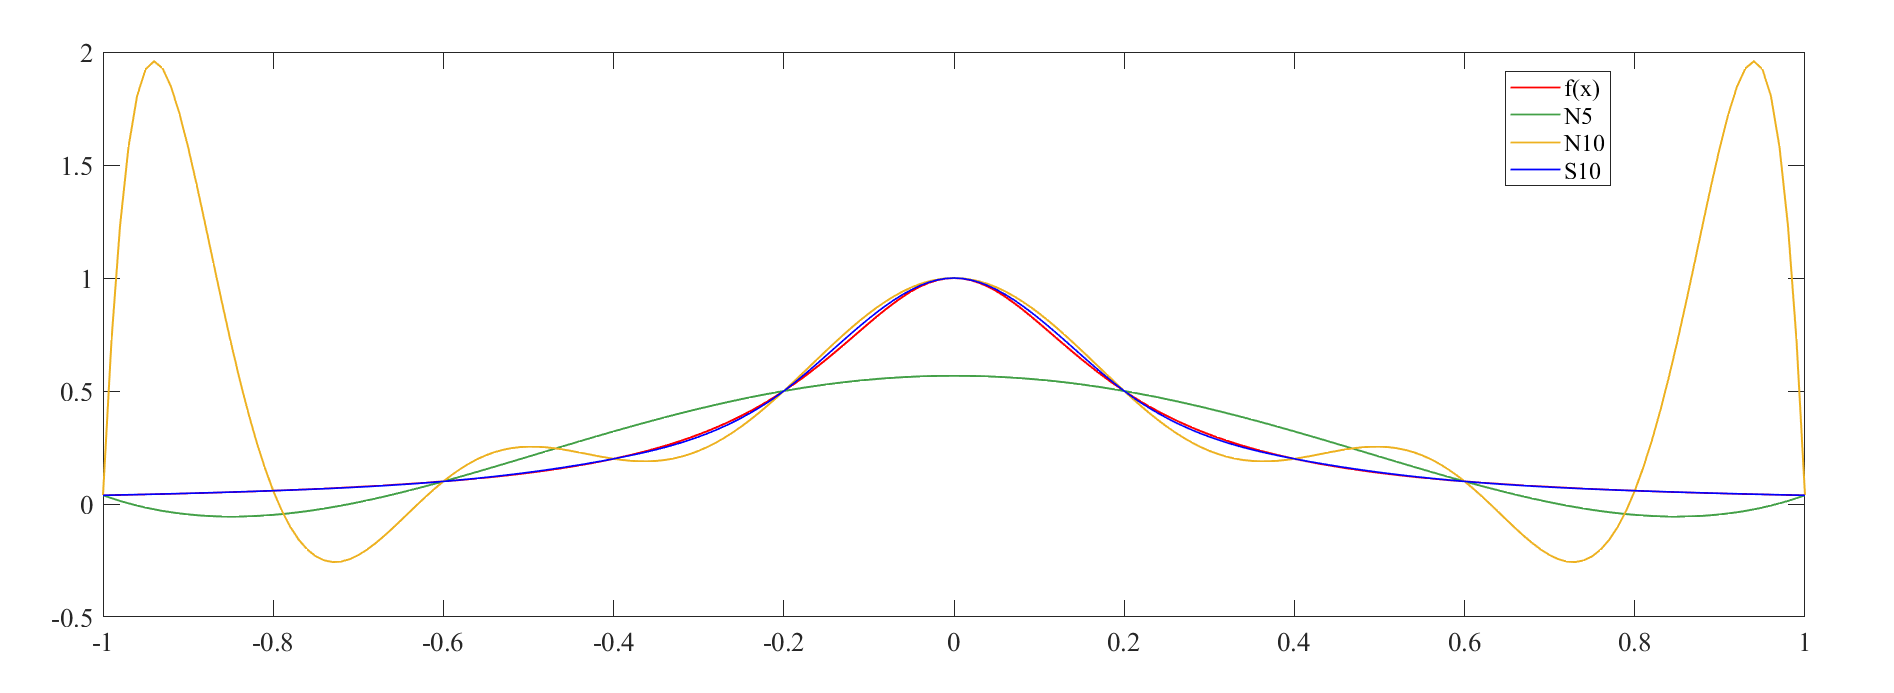
\includegraphics[width=1.2\textwidth]{figure.png}
}

\section{总结}
本次上机实验使我收益颇丰,即使课本已经给出了完整的计算过程,但是要转化为能实际运算的代码还有很多工作要做。由于三次样条插值法涉及的变量较多,首先要分清楚变量之间的推导关系,进而设定每个向量或矩阵的内容和大小,再写出化简后的推导式,有了简化的关系式代码就很容易写出了。

将变量矩阵化转化为矩阵的对应项相乘从而减少代码量的思路是我自己想的,想法来源于曾经写过的$\text{BP神经网络}$问题\footnote{\url{https://wty-yy.github.io/posts/2534/}},但并不能保证这样做是最优的。这里只提供一种思路,也可能由更优秀的写法,请读者多多包容。

由于这是我第一次用$\text{LaTeX}$书写报告,仍有很多生疏的地方,但通过查阅网上的相关资料,基本完成了本次报告,使用$\text{LaTeX}$书写报告虽然开始上手有点困难,但是熟练之后就变得十分轻松了。$\text{LaTeX}$和$\text{Word}$相比,好处在于只要设定好模板,就不用太过于注意排版的细节,直接编译就能获得令人满意的结果。
\newpage
\begin{appendices}
\section{补充\ Chebyshev插值法}\label{sec:buchong}
\subsection{Chebyshev多项式}
\text{Chebyshev}(切比雪夫)多项式为如下形式
\begin{equation*}
    T_k(x)=\cos(k\, \arccos(x)),\quad -1\leqslant x\leqslant 1;\ k=0,1,2,\cdots
\end{equation*}
且有三项递推关系
\begin{equation*}
    T_{k+1}(x) = 2xT_k(x)-T_{k-1}(x),\quad k=1,2,\cdots
\end{equation*}
通过递推式,可知$T_k(n)$的最高次项系数为$2^{n-1}$
\begin{equation*}
    T_0(x) = 1, T_1(x) = x
\end{equation*}

\subsection{算法原理}
观察$\text{Lagrange}$插值多项式余项估计
\begin{equation*}
    R_n(x) = \frac{f^{n+1}(\xi)}{(n+1)!}(x-x_0)(x-x_1)\cdots(x-x_n) = \frac{f^{n+1}(\xi)}{(n+1)!}\pi_{n+1}(x)
\end{equation*}
可知,为了使余项尽可能小,我们期望让$\pi_{n+1}(x)$的最大值尽可能小,而$\text{Chebyshev}$多项式就正好有这个性质:

\begin{property}
    设$p_n(x)$为任意一个首一$n$次多项式,则
    \begin{equation*}
        \max_{-1\leqslant x\leqslant 1}|p_n(x)|\geqslant \max_{-1\leqslant x\leqslant 1}\left|\frac{1}{2^{n-1}}T_n(x)\right|=\frac{1}{2^{n-1}}
    \end{equation*}
\end{property}

通过这个性质可以看出,最高次项相同时,\textbf{首一}的$\text{Chebyshev}$多项式是全体首一多项式中上下界最紧的,也即是最大值最小的,所以如果将$\pi_{n+1}(x)$的$n+1$个零点取成$n+1$次$\text{Chebyshev}$多项式的零点,就可以使得余项最小,从而获得最好的逼近效果。

通过$\text{Chebyshev}$多项式的定义式,不难求出,$T_{n+1}(x)$的$n+1$个零点分别为:
\begin{equation*}
    \frac{(2k+1)\pi}{2(n+1)},\quad(k=0,1,2,\cdots,n)
\end{equation*}

所以只需要将$\text{Newton}$插值法中插值点从均匀点改成$\text{Chebyshev}$多项式的上述零点即可,代码不难实现:

\begin{lstlisting}
    xx = cos((1:2:11)*pi/12)'; % Chebyshev插值T5与平均插值点作比较
    y = Newton(xx, f(xx));
    disp("T5 = ")
    disp(y) % 输出T5的结果
    plot(x, subs(y, x), 'color', '#1E88E5', 'linewidth', 1); % T5图像
\end{lstlisting}

\subsection{试验结果}

将以均匀点的插值函数$N_{10}$,和$6,11$次$\text{Chebyshev}$多项式零点作为插值点所确定的$5,10$次插值函数$T_{5},T_{10}$作比较,可得如下结果
\begin{equation*}
    \begin{aligned}
        T_{5} = &\ 0.71157*x^4 - 1.0958*x^2 + 0.44409\\
        T_{10} =&\ - 46.633*x^{10} + 130.11*x^8 - 133.44*x^6 + 61.443*x^4 - 12.477*x^2  + 1.0\\
        &\ - 39333.0*x^{10} + 12636.0*x^8 - 2537.3*x^6 + 306.63*x^4 - 21.762*x^2 + 1.0
    \end{aligned}
\end{equation*}

\centerline{
    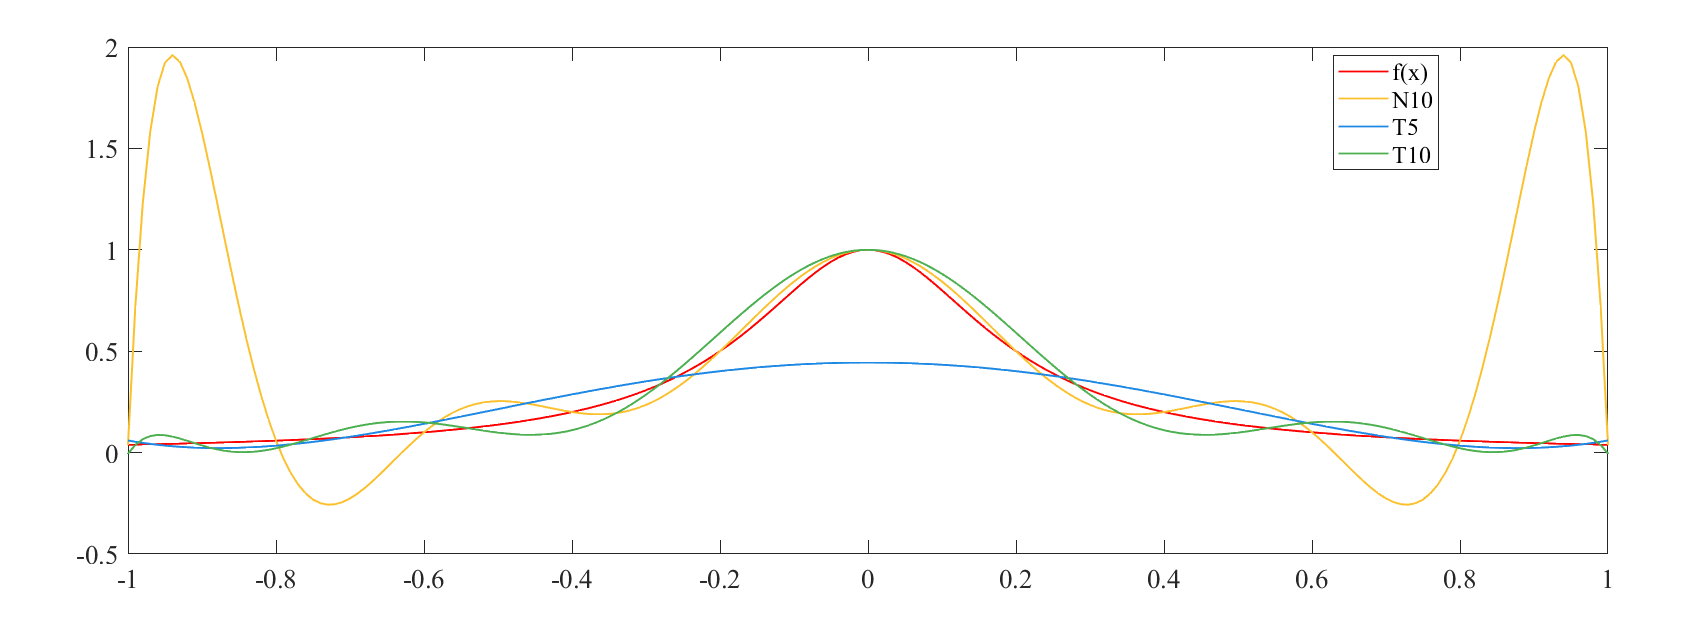
\includegraphics[width=1.2\textwidth]{figure2.png}
}
不难看出,$\text{Chebyshev}$插值法有效的消除了高次插值多项式的$\text{Runge}$现象,是非常有效的改进算法。

\newpage
    \section{代码}\label{sec:fulu}
    可供拷贝的\href{https://paste.ubuntu.com/p/8ddpnhVkTb/}{代码链接}\footnote{\url{https://paste.ubuntu.com/p/8ddpnhVkTb/}},这里也附上完整代码(不包含$\text{Chebyshev}$插值法):
    \begin{lstlisting}
function main
    format short
    a = -1;
    b = 1;
    x = (a:0.01:b)';
    plot(x, f(x), 'r', 'linewidth', 1); % f(x)图像
    hold on
    % Newton插值法求N5,N10
    xx = (a:2/5:b)';
    y = Newton(xx, f(xx));
    class(y)
    disp("N5 = ")
    disp(y) % 输出N5插值结果
    plot(x, subs(y, x), 'color', '#43A047', 'linewidth', 1); % N5图像
    hold on
    xx = (a:2/10:b)';
    y = Newton(xx, f(xx));
    disp("N10 = ")
    disp(y) % 输出N10插值结果
    plot(x, subs(y, x), 'linewidth', 1); % N10图像
    hold on
    % 三次样条插值
    xx = (a:2/10:b)';
    y = mySpline(xx, f(xx), fff(a), fff(b));
    disp("S10 = ")
    disp(y)
    for i = 1 : 10
        l = xx(i);
        r = l + 2/10;
        x = l:0.01:r;
        plot(x, subs(y(i), x), 'b', 'linewidth', 1) % S10图像
        hold on
    end
    legend(["f(x)" "N5" "N10" "S10"]);
    set(gca, 'FontName', 'Times New Roman', 'FontSize', 16);
end

function y = f(x)
    y = 1 ./ (1 + 25 * x .* x);
end
function y = fff(x)
    y = 50 * (75*x.*x-1) ./ (1+25*x.*x)^3;
end

% Newton插值法,a为插值点列向量,b为插值点对应的函数值列向量
function N = Newton(a, b)
    [n, ~] = size(a);
    diff = zeros(n, n); % 初始化差商表
    diff(1, :) = b';
    syms x % 定义参数x
    now = 1; % 对应上文中的 pi(x)
    N = diff(1, 1);
    % 递推计算差商表,并同时计算出插值多项式N(x)
    for i = 2 : n
        for j = i : n
            diff(i, j) = (diff(i-1, j)-diff(i-1, j-1)) / (a(j) - a(j-i+1));
        end
        now = now * (x-a(i-1));
        N = N + diff(i, i) * now;
    end
    N = expand(N); % 展开插值多项式
    N = vpa(N, 5); % 将分式系数转化为小数系数
end

% 三次样条插值法
% a为传入的插值点构成的向量,b为插值点对应函数值构成的向量,M1,Mn为边界条件
function S = mySpline(a, b, M1, Mn)
    [n, ~] = size(a);
    % 向量定义
    h = a(2:n) - a(1:n-1); % 求解向量h
    mu = h(1:n-2) ./ (h(1:n-2) + h(2:n-1)); % 求解向量mu
    la = 1 - mu; % 求解向量lambda
    h1 = h(1:n-2); % 定义中间变量h1
    h2 = h(2:n-1); % 定义中间变量h2
    % 求解向量d
    d = 6*((b(3:n)-b(2:n-1))./h2-(b(2:n-1)-b(1:n-2))./h1)./(h1+h2);

    % 生成系数矩阵A,修改d向量,利用追赶法求解M
    A = zeros(n-2, n-2); % 初始化系数矩阵A
    for i = 1 : n-2 % 循环构造系数矩阵A
        if (i > 1)
            A(i, i-1) = mu(i); % 对角线下方
        end
        A(i, i) = 2; % 对角线
        if (i < n-2)
            A(i, i+1) = la(i); % 对角线上方
        end
    end
    d(1) = d(1) - mu(1) * M1; % 修改向量d
    d(n-2) = d(n-2) - la(n-2) * Mn; % 修改向量d
    M = [M1; chase(A, d)'; Mn]; % 利用追赶法求解方程组,并解出向量M

    % 求解三次样条插值函数S(x)
    syms x % 定义参数x
    % 根据上述定义,计算出以下6个中间变量
    x1 = a(2:n) - x;
    x2 = x - a(1:n-1);
    m1 = M(1:n-1);
    m2 = M(2:n);
    y1 = b(1:n-1);
    y2 = b(2:n);
    % 求解三次样条插值函数
    S = (x1.^3).*m1./(6*h)+(x2.^3).*m2./(6*h)+(y1-h.^2.*m1/6).*x1./h+(y2-h.^2.*m2/6).*x2./h;
    S = expand(S); % 展开插值多项式
    S = vpa(S, 5); % 将分式系数转化为小数系数
end

% 求解三对角方程组的追赶法
function x = chase(A, d) % A为系数矩阵,d为方程组右侧列向量
    [n, ~] = size(A);
    % 预分配内存,提高运算速度
    u = zeros(n, 1);
    l = zeros(n, 1);
    y = zeros(n, 1);
    % 参考课本第36面代码
    u(1) = A(1, 1);
    y(1) = d(1);
    for i = 2 : n
        l(i) = A(i, i-1) / u(i-1);
        u(i) = A(i, i) - l(i) * A(i-1, i);
        y(i) = d(i) - l(i) * y(i-1);
    end
    x(n) = y(n) / u(n);
    for i = n-1 : -1 : 1
        x(i) = (y(i) - A(i, i+1) * x(i+1)) / u(i);
    end
end
    \end{lstlisting}
\end{appendices}

\end{document}

\iffalse
% 图片模板
\centerline{
    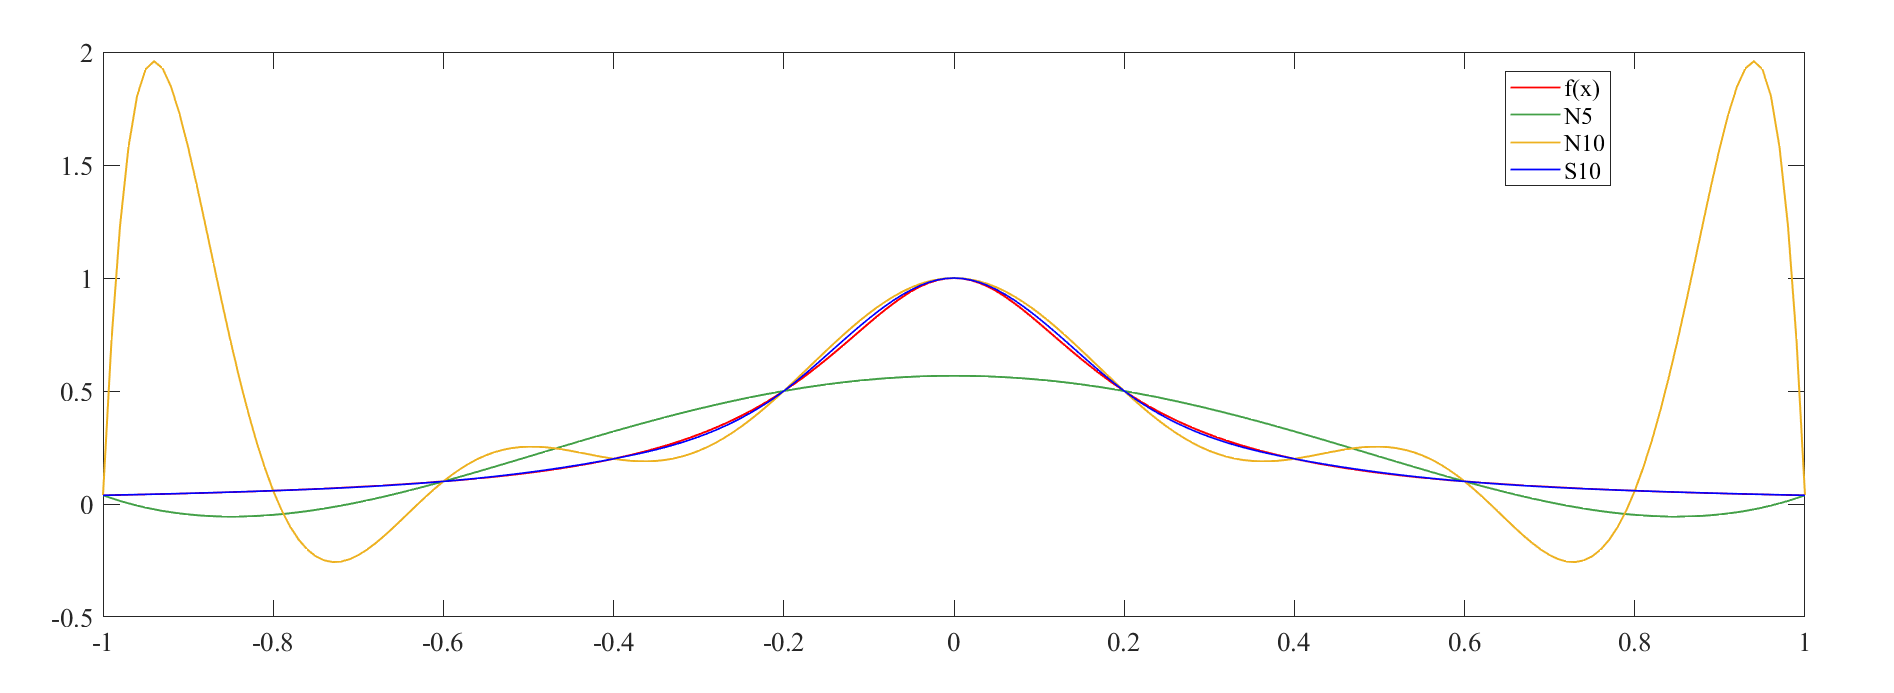
\includegraphics[width=0.8\textwidth]{figure.png}
}
\fi
\iffalse
% 表格模板
\renewcommand\arraystretch{0.8} % 设置表格高度为原来的0.8倍
\begin{table}[!htbp] % table标准
    \centering % 表格居中
    \begin{tabular}{p{1cm}<{\centering}p{1cm}<{\centering}p{3cm}<{\centering}p{5cm}<{\centering}} % 设置表格宽度
    %\begin{tabular}{cccc}
        \toprule
        $x_i$ & $f[x_1]$ & $f[x_i,x_{i+1}]$ & $f[x_i,x_{i+1},x_{i+2}]$ \\
        \midrule
        $x_0$ & $f(x_0)$ &                  &                          \\
        $x_0$ & $f(x_0)$ & $f'(x_0)$        &                          \\
        $x_0$ & $f(x_1)$ & $\frac{f(x_1)-f(x_0)}{x_1-x_0}$ & $\frac{f(x_1)-f(x_0)}{(x_1-x_0)^2}-\frac{f'(x_0)}{x_1-x_0}$\\
        \bottomrule
    \end{tabular}
\end{table}
\fi

\end{document}